%% The following is a directive for TeXShop to indicate the main file
%%!TEX root = diss.tex

\chapter{Sediment transport and landscape evolution}
\label{ch:Introduction}

Landscapes evolve when water, wind, and ice, driven by gravity, erodes down slopes produced by tectonics.
Channels initiate along faults and depressions wherever climatic conditions are suitable, incising networks in the landscape and transferring sediments from uplands to lowlands.
Earth's biota colonize these networks which form conduits for migration, transmitting water, genetic information, and organic material alike, while biota and chemical decomposition convert sediments to soils, staging the joint evolution of life and landscapes which has occurred across geological time.

Human impacts on these old patterns have become severe, in what has been characterized as an environmental and social crisis \citep{Slaymaker2021}.
Research demonstrates unprecedented recent shifts in ancient climatic \citep{Sivan2004,Slater2021}, denundational \citep{Hooke2000,Szabo2010}, and biotic patterns \citep{Walther2002,Willis2009}, requiring effective aquatic habitat restoration, contaminant management, and engineering strategies more than ever before.

In this context river geomorphology as a scientific discipline has shifted toward more quantitative methods that enable concrete predictions about the natural world \citep{Church2005,Church2010}.
Sediment transport in river channels is especially amenable to this quantitative approach since it is mechanistically the result of fluid and granular physics.
Sediment moves in different modes depending on the relative importance of the fluid forces against the weight of grains \citep{Bagnold1956}.
When particles are coarse, as in gravel-bed rivers, the fluid forces are relatively weak and particles move as ``bedload", by bouncing, rolling, and sliding along the bed surface \citep{Kalinske1947}. In bedload transport conditions, fluid turbulence and the irregular bed surface adopt particular control over the sediment dynamics \citep{Ferreira2015}.

Bedload transport exerts unique influence over channel morphology and stability \citep{Church2006,Recking2016}, in part because the coarsest grains in a river provide a partially-immobile skeleton upon which sedimentary deposits can develop \citep{Hassan2008, Eaton2020}.
A longstanding problem in river science is therefore to determine the bedload flux, or the rate of coarse sediment movement.
Unfortunately, existing approaches to compute the bedload flux are inadequate, and predictions often deviate from measured values by orders of magnitude \citep{Gomez1989, Barry2004, Bathurst2007a, Recking2012}.
Given that the problem has been researched intensively for over a century now \citep{Gilbert1914}, it is clear that new research strategies are needed \citep{Ancey2020a,Ancey2020}.

Predicting bedload fluxes is challenging because transport is not always well correlated to average characteristics of the flow and bed material. 
Local fluxes can range through orders of magnitude as details of turbulent fluctuations and bed organization vary, while average characterizations of flow and sediment remain constant \citep{Sumer2003, Charru2004, Hassan2008, Venditti2017}.
The same turbulence and sediment organization details which correlate with the bedload flux are also modified by it.
Turbulent impulses drive sediment motion \citep{Valyrakis2010, Celik2014, Amir2014, Shih2017}, but moving sediment affects turbulent flow characteristics \citep{Singh2010, Santos2014, Liu2016}. The surface arrangement and consolidation of grains \citep{Miller1966,Paintal1971,Dwivedi2012} affects sediment mobility, but transport rearranges grains and consolidates the bed \citep{Kirchener1990, Charru2004, Allen2018, Masteller2019, Pretzlav2020}.
Bedload fluxes are in cyclical feedback with their controls \citep{Jerolmack2005}, and this challenges us to step beyond descriptions based on averaged values \citep{Ancey2020b}.

The approach taken in this thesis is to consider bedload transport as an aggregate result of many individual transported grains whose movements have probabilistic characteristics.
This departs from the traditional strategy of correlating transport rates to the average flow and sedimentary characteristics \citep{MeyerPeter1948, Parker1990, Wilcock2001}.
Because the trajectories of individual grains are governed by Newtonian mechanics, this approach brings powerful tools to the problem, but it is nonetheless complicated because the forces driving and resisting sediment motion vary through space and time due to fluid turbulence and the erratic interactions of moving particles with the bed.


To address these complications, I develop in this thesis a handful of new bedload transport models using methods adopted from statistical physics.
To provide context and motivation, the thesis begins by reviewing earlier approaches to bedload transport which my work is most related to, rephrasing works as necessary during this review to indicate common themes and show continuity with my own developments which follow in subsequent chapters.

\section{Theories of individual particle movement}
\label{sec:trajmodels}

A basic problem in sediment transport theory is to predict the downstream movement of individual particles.
At first glance, this seems an elementary problem in general physics, but numerous challenges appear.
Particles moving as bedload are driven downstream by a turbulent fluid flow, but the exact relationships between the fluid flow and the applied forces are not exactly known \citep{Maxey1983,Schmeeckle2007}.
Downstream movement is resisted by frictional encounters (skidding, pivoting, colliding) between moving particles and the bed, but since the bed is a granular surface, its geometry is difficult to characterize \citep{Gordon1972}, and the role of bed interactions is challenging to describe \citep{Sekine1992, Nino1998}.

Entrainment and deposition provide an additional layer of complexity.
Moving particles that encounter the bed with sufficiently low velocities can settle into pockets which protect them from the flow \citep{Miller1966} and cause deposition \citep{Charru2004}.
These pockets are not permanent shelter because rearrangement of the surrounding bed by entrainment of neighboring particles or subsurface creep \citep{Houssais2016,Frey2014} can re-expose particles to the flow, and sufficiently strong turbulent fluctuations \citep{Cameron2020} can overcome shelter even if its geometry is not disturbed \citep{Valyrakis2010,Celik2014}. 
As a result, particles generally alternate through sequences of entrainment and deposition, but the exact times at which these alternations occur is difficult to characterize \citep{Einstein1937}.

Particles at rest on the bed surface can also become covered by other transported particles \citep{Yang1971}. 
These buried particles cannot move again until those burying them have been transported away \citep{Nakagawa1981}, generating long periods of immobility \citep{Hassan1994,Ferguson2002}.

Individual trajectories of particles therefore involve a number of contributing processes which occur over different characteristic timescales, from seconds to years \citep{Pretzlav2021}, and each of these processes has so far evaded any exact description.

\citet{Nikora2001,Nikora2002} provided a conceptual framework which helps to organize this complexity.
Nikora et al divided the downstream tractories of individual particles into three timescales, or ``ranges", termed local, intermediate, and global.
The local range refers to the period of motion between subsequent interactions with the bed, when the particles accelerate downstream within the turbulent flow.
The intermediate range reflects particle motions through sequences of bed encounters, when particles alternately accelerate and decelerate. 
The global range refers to particle trajectories through sequential entrainment and deposition events as they cycle between motion and rest.
\citet{Hassan2017} added an additional range, referred to as ``geomorphic", to reflect the even longer period over which particles become buried within the subsurface or embedded among sedimentary deposits \citep{Bradley2017}.
This set of timescales -- local, intermediate, global, and geomorphic -- are used below to organize the literature describing trajectories of individual grains.

\subsection{Motivation: tracers and basic understanding}
An early motivation to understand individual particle motions was to predict the efficiency of sediment transport measurements \citep{Ettema2004}, and this motivation still drives a great deal of research into individual particle motions today \citep{Hassan2017,Pretzlav2021}.
A common technique to estimate sediment transport is to seed a stream with tracer stones and track their progress downstream \citep{Einstein1937, Takayama1965, Pretzlav2021}.
In principle, tracers provide a proxy for the population of grains in a stream, so one can estimate tracer velocities of tracers, then multiply by an estimate of the number of grains available for motion to calculate the overall sediment flux \citep{Wilcock1997a,Ferguson2002}.
In practice, challenges arise due to the distinct behavior of tracers over the local, intermediate, global, and geomorphic timescales. Apparently, tracer velocities depend on the observation time, in a phenomenon which has been called ``advective slowdown" \citep{Ferguson2002,Haschenburger2011, Haschenburger2013, Pelosi2016}. This obscures the relationship between measured tracer velocities and actual sediment fluxes, exposing a need for further research into how exactly individual particle motions depend on observation scale and what processes generate advective slowdown.

\subsection{Einstein's random walk model}
\label{sec:einwalk}
Einstein was probably the first to model the movements of individual particles through streams \citep{Einstein1937}.
Watching painted tracers move through a flume, Einstein came to the conclusion that the movement characteristics of any one particle could not be predicted, so he turned to probabilistic methods to characterize their transport.

Einstein's key insight was to represent particle motions as an alternating sequence of movements and rests having random characteristics.
As his interest was on the global range of particle motion when many motion-rest alternations have occurred, and because the duration of particle motions is usually short compared to rests, Einstein made the approximation that individual motions (between entrainment and deposition) are mathematically instantaneous.
With this approximation, the downstream movement of sediment becomes an alternate cycle of instantaneous steps of random length, separated by rests of random duration. 
Implicitly, this picture of sediment trajectories assumes that movement velocities are infinite.

Einstein's experiments indicated that both step lengths and resting times were well-described by exponential distributions, and the focus of his PhD was to find the probability density $P(x,t)$ that a particle had travelled a net distance $x$ after a time $t$ has elapsed. In the course of this research, Einstein formulated an example of what is now called the continuous time random walk, but this was not formalized until much later \citep{Montroll1965}.

Einstein's assumptions imply that if the position of a single sediment particle at a given time is $x(t)$, the assumptions of infinite movement velocity, random resting durations, and random movement distances between entrainment and depositon (step lengths) can be written
\be \dot{x}(t) = \mu(t), \label{eq:einlangevin}\ee
where $\dot{x} = dx/dt$, and $\mu(t)$ is a white shot noise \citep{VanDenBroeck1983}, which is essentially a sequence of pulses having random heights with mean height $\ell$ (the mean step length), and random locations in time with mean separation $1/k_E$ (the mean resting time, interpreted as the reciprocal of the entrainment rate $k_E$).
A particular realization of this pulsed noise can be written
\be \mu(t) = \sum_{i=1}^{N(t)}s_i \delta(t-t_i). \label{eq:einrando} \ee
Here $N(t)$ is the number of particle entrainments in time $t$ which is  a Poisson random variable, distributed as $P(N) = e^{-k_E t} (k_E t)^N/N!$.
The $t_i$ are distributed according to $P(t) = k_E\exp(-k_E t)$, and the $s_i$ are step lengths distributed according to $P(s) = \ell^{-1}\exp(-s \ell^{-1}).$
Figure \ref{fig:einsteinfig} panel (a) sketches the pulsed noise $\mu(t)$, and panel (b) sketches the resulting global range bedload sediment trajectories as a sequence of steps and rests.

Equation \ref{eq:einlangevin} is a kind of dynamical equation representing how the position of a sediment grain evolves through time \citep{Kubo1978}, similar to Newtonian mechanics \citep{Goldstein1997} but with random driving term (equation \ref{eq:einrando}).
\begin{figure}[!htbp]
	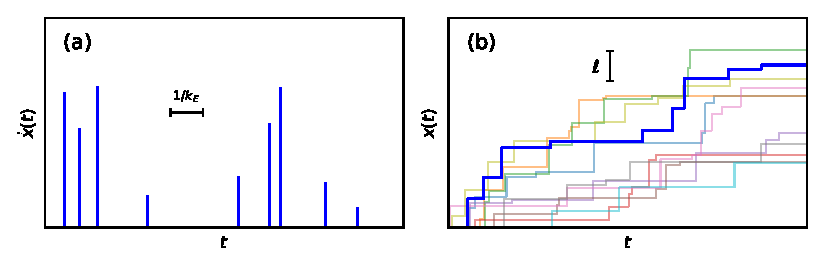
\includegraphics[width=\linewidth,keepaspectratio]{./figures/ch1/einsteinConcept.pdf}
	\caption{Panel (a) indicates the representation of Einstein's model as an idealized ``white shot noise", as indicated in eq. \ref{eq:einrando}, while panel (b) shows the ``stairstep" trajectories of sediment particles moving downstream through cycles of steps (which are instantaneous) and rests (which have mean duration $1/k_E$). }
	\label{fig:einsteinfig}
\end{figure}

The governing equation of the distribution $P(x,t)$ to find the particle at $x$ can be calculated as an ensemble average of $\delta(x-x(t))$ over all possible realizations of the noise \citep{Risken1989,Moss1989}. Different methods exist to compute such averages \citep{Hanggi1978, Hanggi1984a, Balakrishnan1993, VanDenBroeck1983}, but whatever the approach, the governing equation for the distribution comes out as
\be  \big(\ell \px \pt + k_E \ell \px + \pt \big)P(x,t) = 0. \label{eq:einmaster}\ee
This equation can be solved by standard methods (series solutions or transform calculus) \citep{Arfken1985,Prudnikov1992a} to reproduce the original result of \citet{Einstein1937} for the probability distribution of position of a sediment particle:
\be P(x,t) = \Big[\delta(x) e^{-k_E t} + e^{-k_E t - x/\ell} \sqrt{\frac{k_E t}{\ell x}}\mathcal{I}_1\Big(2 \sqrt{\frac{k_E x t}{\ell}}\Big)\Big]\theta(x)\theta(t) \label{eq:eindist} \ee
Here, $\mathcal{I}_\nu$ is a modified Bessel function of order $\nu$. 
The probability distribution eq. \ref{eq:eindist} fully characterizes the downstream movement of an individual particle alternating randomly through steps and rests.

This distribution displays both advection and diffusion. Advection occurs because particles move downstream. Diffusion occurs because step lengths and instants when entrainment events occur vary from one particle to the next.

One can calculate all moments of the position by multiplying eq. \ref{eq:einmaster} by $x^n$ and integrating over space. This gives the mean position of the particle
\be \langle x (t)  \rangle = k_E \ell t. \ee
This equation indicates that in Einstein's model, sediment grains move with effective velocity $V_\text{eff} = k_E \ell$ given by the product of the entrainment rate and mean step length.

The rate at which particles spread apart due to differences in their trajectories can be represented by the variance of position, $\sigma_x^2  = \langle x^2 \rangle - \langle x \rangle^2$. This gives
\be \sigma_x^2(t) = 2 k_E \ell^2 t, \ee
so particles in Einstein's model spread apart as a normal diffusion process $\sigma_x^2 = 2 D_\text{eff} t$ \citep{Sokolov2012}, with an effective diffusivity $D_\text{eff} = k_E \ell^2.$

\subsection{Inclusion of the movement duration}
\label{sec:lisle}

Einstein's model provides an adequate description of global range particle transport when the period of interest is much larger than the timescales of individual particle movements (local and intermediate ranges) and much smaller than the timescales over which particles become embedded in sedimentary deposits (geomorphic range).

The advent of high speed camera experiments produced new insight into the local and intermediate ranges of bedload motion \citep{Abbott1977,Francis1973,Drake1988} which \citet{Einstein1937} never intended for his model to describe.
In the local range, particles move with a fluctuating velocity due to the variable drag of the turbulent flow \citep{Lajeunesse2010,Fathel2015} and changes in the particle's height within the flow profile \citep{VanRijn1984,Wiberg1985}.
In the intermediate range, particle-bed collisions impart additional variability to sediment velocities \citep{Gordon1972,Martin2013}.
Einstein's instantaneous movement assumption obscures the timescales over which these processes occur.

Studies by \citet{Lisle1998}, and \citet{Lajeunesse2017} generalized the Einstein theory to include intermediate timescales. They approximated particle velocities as constant (neglecting fluctuations), and assumed that the movement times are exponentially distributed random variables just like resting times, but this time characterized by a deposition rate $k_D$, whose reciprocal is the average period of time a particle spends in motion between entrainment and deposition.
The analogue of Einstein's model equation \ref{eq:einlangevin} with a finite movement velocity $V$ can be written
\be \dot{x} = V\eta(t), \label{eq:lislelangevin}\ee
%where the noise is now a ``dichotomous Markov noise" \citep{VanDenBroeck1990,Bena2006}, which is essentially a random switch or telegraph signal that alternates between ``on" ($\eta(t) = 1$, meaning the particle is moving) and ``off" ($\eta(t) = 0$, meaning the particle is resting) \citep{Cox1965,Horsthemke1984, Masoliver1991, Masoliver1996}.
This noise is displayed in figure \ref{fig:lislefig} panel (a). Some particle trajectories produced by equation \ref{eq:lislelangevin} are displayed in figure \ref{fig:lislefig} panel (b).

The governing equation of the position probability distribution $P(x,t) = \langle \delta(x-\int_0^t V\eta(t')dt') \rangle$ becomes \citep{Balakrishnan1993}
\be \big(\pt^2 + V \px \pt + k_E V \px + k \pt \big) P(x,t) = 0,\label{eq:lislemaster}\ee
where $k_E$ and $k_D$ are the entrainment and deposition rates, $V$ is the particle velocity during the motion state, and $k = k_E+k_D$. This partial differential equation is called an asymmetric telegrapher's equation \citep{Rossetto2018}, and although the symmetric analogue of this equation is well-studied \citep{Weiss2002a, Masoliver2017}, the asymmetric problem is not often encountered.
\begin{figure}[!htbp]
	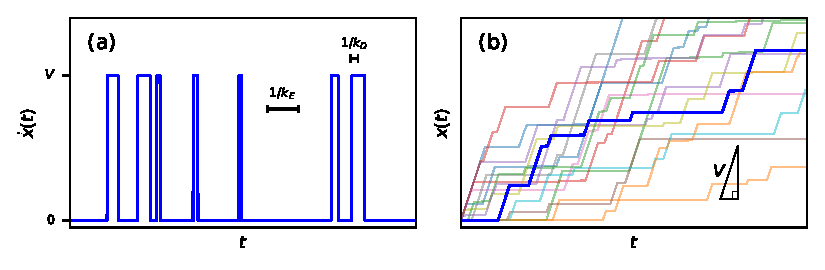
\includegraphics[width=\linewidth,keepaspectratio]{./figures/ch1/lisleConcept.pdf}
	\caption{Panel (a) indicates the generalization of Einstein's model to include the interval of sediment motion between entrainment and deposition, now represented with dichotomous noise eq. \ref{eq:lislelangevin}, while panel (b) shows the tilted stair-step trajectories of sediment particles moving downstream in cycles of motion at velocity $V$ (with mean duration $1/k_D$) and rest (with mean duration $1/k_E$). }
	\label{fig:lislefig}
\end{figure}

For the initial condition that particles have a probability $k_E/k$ to start in motion, reflecting steady state conditions as far as alternation between motion and rest are concerned \citep[e.g.][]{Ancey2006}, the solution of equation \ref{eq:lislemaster} is \citep{Lisle1998}
\begin{multline}  P(x,t) =  e^{-\chi-\tau} \Big[ \frac{k_E}{V}\delta(\tau) + \frac{k_E}{V} \sqrt{\frac{\chi}{\tau}}\mathcal{I}_1(2\sqrt{\chi\tau}) + \frac{k_D}{V}\mathcal{I}_0(2\sqrt{\chi\tau}) \\
	+ \frac{k_Ek_D}{kV}\sqrt{\frac{\tau}{\chi}}\mathcal{I}_1(2\sqrt{\chi\tau}) + \frac{k_Ek_D}{kV} \delta(\chi)
	\Big]\theta(\chi)\theta(\tau), \label{eq:lisledist}
\end{multline}
where $\chi = k_D x/V$ and $\tau = k_E(t-x/V)$ are shorthand notations.
Incorporating the duration of sediment motion, the mean position of the sediment grain remains linear in time: $\langle x (t) \rangle  = k_E V t/k$, representing movement with an effective velocity $V_\text{eff} = k_E V/k$, which is the fraction of time spent in motion ($k_E/k)$ \citep{Ancey2006} multiplied by the velocity during the motion state. In contrast, the variance develops a two range scaling.
Computing $\sigma_x^2$ provides
\be \sigma_x(t)^2 = \frac{2k_Ek_DV^2}{k^3}\Big( t + \frac{1}{k}e^{-k t} - \frac{1}{k}\Big) , \label{eq:lislevar}\ee
which is a non-trivial result. At short times, for $t\ll 1/k$, equation \ref{eq:lislevar} shows diffusion $\sigma_x^2 \sim t^2$, which is a faster ``ballistic" rate of spreading than the Einstein model predicts \citep{Sokolov2012}. At long times ($t\gg 1/k$), the diffusion becomes normal again ($\sigma_x^2 = 2 D_\text{eff} t$), with an effective diffusion constant $ D_\text{eff} = k_E k_D V^2/k^3$. 
The rapid spreading of particles at short timescales occurs because some are completely stationary while others move with velocity $V$.

The eventual transition to normal diffusion occurs because particles eventually become well-mixed among motion and rest states. An analogous diffusion phenomenon is described in \citet{Taylor1920}.

In this trajectory model, both intermediate and global ranges are adequately represented, but local and geomorphic are not, the former since fluctuations of the velocity between entrainment and deposition have been neglected, and the latter since particle burial was not incorporated.

\subsection{The Newtonian approach}

Some authors have modelled local and intermediate ranges of individual particle trajectories by writing approximate Newtonian equations for the dynamics of individual particles and integrating them numerically. Early efforts applied time-averaged fluid forces linked to the logarithmic mean flow velocity profile \citep{Yalin1963,VanRijn1984}, and later efforts included collision models to modify particle velocities upon bed contact \citep{Wiberg1985,Sekine1992,Nino1998}.

Researchers eventually included realistic granular interactions in many-particle simulations of bedload transport using the discrete element method \citep{Cundall1979a, Haff1993}.
The early works utilizing this approach used a two dimensional domain with a highly simplified ``slab" flow model \citep{Haff1993}, while later works have included synthetic turbulence to drive particles \citep{McEwan2001,Schmeeckle2003,Maurin2015} or clever reduced-complexity representations of the flow \citep{Clark2015,Clark2017}.

The state of the art within this category of sediment transport models is to include two-way coupling between particles and the fluid flow. The latter is modelled either by large eddy simulation or direct numerical simulation of the Navier-Stokes equations, while particles provide the boundary condition for the flow \citep{Schmeeckle2014,Ji2013,Gonzalez2017,Vowinckel2014,Elghannay2017,Yousefi2020}.
These computational physics models produce impressive insight into the underlying granular and fluid physics mechanisms producing bed load transport \citep{Frey2011}, but analytical models are nevertheless desired for further insight into the problem.

\subsection{Mechanistic-stochastic models for the sediment velocity distribution}
\label{sec:langevin}

Another category of models have described bedload particle velocities using Langevin equations \citep{Ancey2014,Fan2014}, whereby the particles dynamics are driven by Gaussian white noise \citep{Kubo1978}.

Experimental studies on bedload velocities have provided two major conclusions for the shape of the particle velocity distribution. One subset of observations shows that bedload velocities follow exponential distributions \citep{Lajeunesse2010,Furbish2012,Fathel2015}, and another subset shows Gaussian distributions \citep{Martin2012,Ancey2014,Heyman2016}.

\citet{Fan2014} set out to describe exponenential-distributed bedload particle velocities ($u$) with the Langevin equation
\be \dot{u}(t) = -\Delta \text{sgn}(u) + F + \sqrt{2D}\xi(t). \label{eq:fanlangevin}\ee
This equation drives the particle velocity by a fluid drag $F + \sqrt{2D} \xi(t)$, where $F$ is a constant, $D$ is a diffusivity that characterizes the magnitude of drag fluctuations, and $\xi(t)$ is a Gaussian white noise with unit variance and vanishing mean \citep{Gardiner1983}.
This drag is resisted by a heuristic particle friction term $-\Delta \text{sgn}(u)$, introduced as a proxy for particle-bed collisions.
The ``Fokker-Planck equation" governing the probability distribution $P(u,t)$ of the particle velocity can be derived from equation \ref{eq:fanlangevin} as \citep{Risken1989,VanKampen2007} 
\be \frac{\partial}{\partial t} P(u,t) = -\Delta\frac{\partial}{\partial u}\Big[ \text{sgn}(u) P \Big] + D \frac{\partial^2 P}{\partial u^2},\ee
implying that the steady-state velocity distribution ($\pt P(x,t) = 0$) provided by equation \ref{eq:fanlangevin} is
\be P(u) = \frac{\Delta^2-F^2}{2\Delta D}\exp\Big(-\frac{-\Delta |u| + F u}{D}\Big).\ee
This is the (two-sided) exponential distribution observed in one subset of experiments.

\citet{Ancey2014} formulated a Langevin equation to describe the Gaussian velocity distributions observed in the other subset of experiments. They wrote for the streamwise velocity 
\be t_r \dot{u}(t) = -(U-u) + \sqrt{2D}\xi(t),\ee
where $U$ is the mean velocity of particles, $D$ characterizes the magnitude of velocity fluctuations, and $\xi(t)$ is again a Gaussian white noise with vanishing mean and unit variance. The timescale $t_r$ is a relaxation time over which velocity fluctuations decay. This time, the Fokker-Planck equation is
\be \frac{\partial}{\partial t} P(u,t) = -\frac{\partial}{\partial u}\Big[\frac{U-u}{t_r}P\Big] + \frac{D}{t_r^2}\frac{\partial^2 P}{\partial u^2},\ee 
and the steady state solution becomes
\be P(u) = \sqrt{\frac{t_r}{2\pi D}} \exp\Big(-\frac{t_r(u-U)^2}{2 D}\Big), \ee
which is the Gaussian velocity distribution from the other subset of the experiments.
These two models of bedload velocity distributions are summarized in figure \ref{fig:fanAncey}.
\begin{figure}[!htbp]
	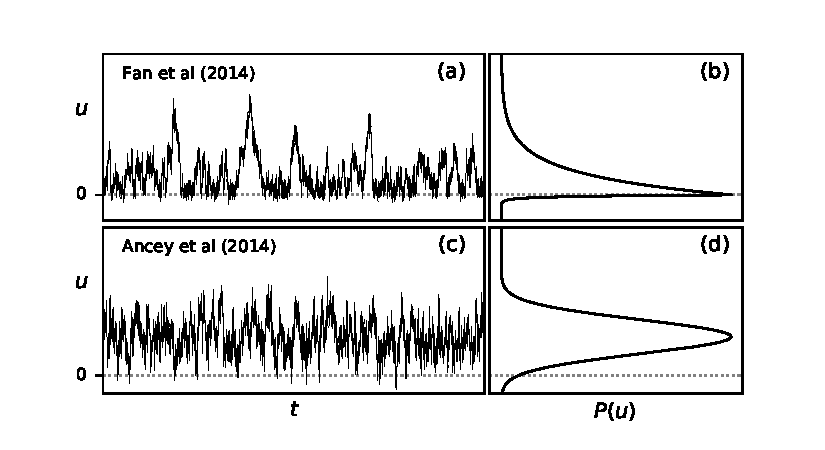
\includegraphics[width=\linewidth,keepaspectratio]{./figures/ch1/fanAncey.pdf}
	\caption{Panel (a) demonstrates the trajectory of a particle within the Fan et al model, where Coulomb friction impedes turbulent drag. Panel (b) shows the resulting exponential particle velocity distribution, having relatively large fluctuations with mode at $u=0$.
	Panel (c) shows the analogous trajectory from the Ancey et al model, where turbulent Stokes drag generates the Gaussian velocity distribution seen in (d). The latter has relatively narrow and symmetric fluctuations, with a positive mode well above $u=0$.}
	\label{fig:fanAncey}
\end{figure}
Although these descriptions describe two end-member sediment velocity distributions, Gaussian and exponential, the underlying mechanical reason why bedload transport has shown multiple velocity distributions remains an open question, and other distributions have been reported besides exponential and Gaussian \citep[e.g.][]{Houssais2012,Liu2019}.
A comprehensive model of the full range of bedload transport observations is a desirable target.

\subsection{The definition of the flux}
\begin{figure}[!htbp]
	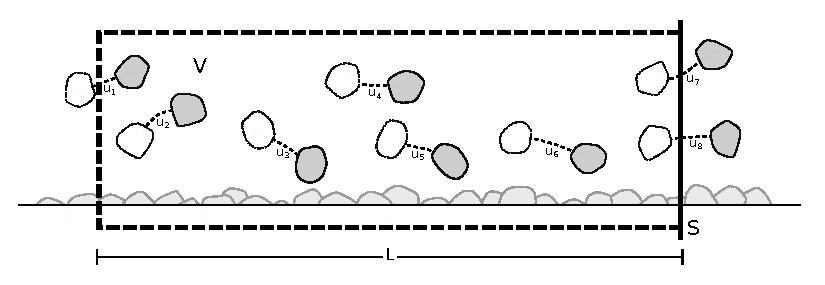
\includegraphics[width=\linewidth,keepaspectratio]{./figures/ch1/fluxDefinitions.pdf}
	\caption{Particle fluxes can be defined with either a control volume $V$ or a control surface $S$. Here, particles are shown moving from time $t-dt$ (faint white particles) to time $t$ (grey particles). Each particle's velocity component $u_i$ in the downstream direction is indicated. At the instant $t$, the surface definition of the flux \ref{eq:surfflux} gives $q = \frac{1}{L}(u_7+u_8).$, while the volume definition \ref{eq:controlflux} gives $\Phi = \frac{1}{L}(u_1+\dots+u_6)$,
	showing the non-equivalence of these two definitions.}
	\label{fig:fluxdefs}
\end{figure}
Perhaps a surprising summary of bedload transport research is that no one definition of the sediment flux has even been agreed upon despite over a century of research \citep{Ballio2018}.
Today, there are two main complementary definitions of the bedload flux. 

The first definition is reminiscent of continuum mechanics and formulates the flux as a kind of current of sediment across a control surface $S$ \citep{Furbish2012,Heyman2016, Ballio2014}: 
\be q = \int_S c(\textbf{x},t)\textbf{u}\cdot d\textbf{S}. \label{eq:surfflux} \ee
This definition involves the concentration $c$ of particles in space and their velocites at the instant they cross the control surface, which is a somewhat elusive quantity since bedload particles are not a continuous field \citep{Heyman2016}.

The second definition formulates the downstream flux in terms of the number of particles moving within a control volume $V$:
\be \Phi = \frac{1}{L} \sum_{i\in V} u_i. \label{eq:controlflux}\ee
Here, the flux is evaluated as a sum over all downstream velocities of particles within the volume (of which there are a fluctuating number), and the division by the downstream length of the control volume is incorporated to count only that proportion of particles near the downstream boundary of the volume. These two definitions, $q$ defined with a surface and $\Phi$ defined with a volume, are generally not equivalent \citep{Ancey2020a}.

\subsection{The scaling arguments of Bagnold}
\label{sec:baggo}

One of the most influential formulations of the bedload flux is due to \citet{Bagnold1956,Bagnold1966}, who derived a formula for the mean sediment flux using an energy balance approach.
Bagnold understood sediment transport as a process which converts flow energy to heat via the effective friction \citep{Bagnold1954} of grains against the bed as they move downstream through a succession of collisions \citep{Bagnold1973}.
He assumed that the flow power $P_f$ available to move sediment in a volume scales as $P_f \propto \tau - \tau_c$, where $\tau$ is the average bed shear stress and $\tau_c$ is the threshold shear stress at which particles first begin to move. 
Considering that the average volumetric flux of particles is $\Phi$, and particles move with mean velocity proportional to the fluid velocity near the bed, Bagnold hypothesized that the power $P_g$required to sustain particle motion in a volume scales as $P_g \propto \Phi/\tau^{1/2}.$
Balancing flow energy against frictional dissipation ($P_f = P_g$) then provides Bagnold's sediment transport formula
\be \Phi = k(\tau-\tau_c)\tau^{1/2}, \label{eq:bagnold}\ee
which has shown good correspondence with laboratory data at large transport rates, given careful calibration of the constant factors $k$ and $\tau_c$.

The large shear stress limit $\Phi \sim \tau^{3/2}$ of Bagnold's formula is shared in common with many other empirical formulas describing the mean downstream flux of bedload \citep[e.g.][]{MeyerPeter1948, Yalin1972, Wilcock2003, Parker1990}. A distinguishing feature of Bagnold's formula is its derivation from mechanistic reasoning, although many of Bagnold's assumptions have since turned out to be incorrect.
Bagnold's assumption that the power available to move sediment scaled with the excess shear stress leads to unphysical results over arbitrarily sloping beds \citep{Seminara2002}, and the flow power dissipated by sediment transport shows only a weak correlation the sediment flux \citep{Ancey2008}, while Bagnold assumed they were directly proportional. These issues have been hinted when calibrating Bagnold's formula to data, where the parameters $k$ and $\tau_c$ take on unphysical values at low transport rates \citep{Nino1996}.
Bagnold's formulation also faces the notorious challenge of defining the critical shear stress $\tau_c$ for the initiation of sediment transport \citep{Paintal1971,Kirchener1990,Houssais2015,Clark2017,Allen2018}.
The difficulties with Bagnold's approach led to many revisions of his theory, often based on more carefully incorporating the properties of individual particle motions into the sediment transport energy budget \citep{Engelund1976,Luque1976,Nino1998,Martin2000}.

\subsection{Einstein's probabilistic approach}
\label{sec:einflux}

Among these revisions of Bagnold, one category shows a return to the probabilistic ideas of Einstein \citep{Parker2003,Ancey2006}.
\citet{Einstein1937} formulated his original model of individual particle trajectories in terms of entrainment and deposition rates using the idealization of grains moving downstream through a sequence of instantaneous steps.
Later, \citet{Einstein1942,Einstein1950} calculated the sediment flux with these same probabilistic ideas, providing an alternative to Bagnold's scaling approach.
The conceptual picture that Einstein considered is depicted in figure \ref{fig:einsteinFluxConcept}.
 \begin{figure}[!htbp]
	\includegraphics[width=\linewidth,keepaspectratio]{./figures/ch1/yalinDrawing.pdf}
	\caption{Einstein’s conceptual picture (modified from \citet{Yalin1972}). Particles move in discrete jumps of length $\ell$ from
left to right through an array of adjacent control volumes. The bedload flux is the rate of particles crossing
the surface $S$ per unit width and time, collected from all upstream control volumes.}
	\label{fig:einsteinFluxConcept}
\end{figure}

Einstein partitioned the channel into a sequence of identical control volumes $V$, and calculated the average rate at which particles cross a control surface by aggregating the contributions from each upstream control volume.
Each control volume has downstream length $\ell$ which is also the average particle step length.
Denoting by $P_n$ the probability that an individual grain undergoes at least $n$ jumps of length $\ell$ in a time interval $T$, meaning it travels at least a distance $n \ell$, and considering that there is a density $\rho$ of particles at rest on the bed, it follows that on average $\rho \ell P_n$ particles will displace a distance $n \ell$ or more from within each control volume during the time interval $T$. 
As a result, since grains crossing $S$ in a time $T$ could have come from any upstream location, the number of grains crossing $S$ in $T$ is a sum over all control volumes: $\sum_{n=1}^\infty \rho \ell P_n$.
Dividing by the time $T$ to get the average rate of grains crossing $S$ provides the mean flux:
\be q = \frac{\rho \ell}{T} \sum_{n=1}^\infty P_n. \label{eq:einflux} \ee
The final quantity to evaluate is $P_n$, the probability a particle entrains \textit{at least} $n$ times in a time $T$.

Einstein originally constructed this probability by assuming that each particle had $n$ independent entrainment opportunities in the period $T$, each with probability $p$, so that $P_n = p^n$, giving $q \propto p/(1-p)$ by a geometric series, but this approach has been criticized by \citet{Yalin1972} and others \citep{Paintal1971,Cheng2004,Armanini2015,Armanini2017}. Some authors have argued convincingly that instead, one should calculate $P_n$ as an exceedance probability.
The central critique is that there is a distinct difference between \textit{exactly} and \textit{at least} $n$ entrainment events in $T$.

If the entrainment rate of an individual grain is $k_E$ (probability per unit time), then the probability that it entrains \textit{exactly} $n$ times in time $T$, denoted by $p_n$ (distinct from $P_n$) is a Poisson distribution \citep{Cox1965}:
\be p_n = \frac{(k_E T)^n}{n!}e^{-k_E T}.\ee
This implies that the probability that it entrains \textit{at least} $n$ times is $P_n = \sum_{i=n}^\infty  \frac{(k_E T)^n}{n!}e^{-k_E T}, $
so Einstein's mean sediment flux across the control surface (eq. \ref{eq:einflux}) becomes
\be q = \frac{\rho \ell}{T} \sum_{n=1}^\infty \sum_{l=n}^\infty = \frac{\rho \ell}{T}\sum_{n=1}^\infty n \frac{(k_E T)^n}{n!}e^{-k_E T} = \rho k_E \ell.\ee
Noticing that $\rho k_E$ is the entrainment rate of a single grain multiplied by the density of grains available for entrainment on the bed, we can summarize the Einstein theory as 
\be q = E \ell, \ee
where the quantity $E = \rho k_E$ is differentthe ``areal entrainment rate", representing the number of grains entrained per unit streambed area \citep{Wilcock1997a,Furbish2012}.

Einstein's formulation requires expressions of the single particle entrainment rate $k_E$ and step length $\ell$ in terms of the flow and sediment characteristics.
Although Einstein and many followers have attempted to formulate these connections \citep[e.g.][]{Einstein1950,Grass1970,Paintal1971}, there are still no comprehensive solutions. Linking Einstein's entrainment and deposition rates to the grain scale mechanics remains an active area of research \citep[e.g.][]{Tregnaghi2012,Dey2018}.

\subsection{Fusing Einstein and Bagnold: The erosion-deposition model}

One uniquely successful strategy to relate Einstein's model to flow and sediment characteristics was developed by \citet{Charru2004,Charru2006}. This ``erosion-deposition model" phrases sediment transport as a mass balance within a control volume using Einstein's entrainment rate $E$ and the complementary deposition rate $D$. These model parameters are related to flow and sediment properties using scaling relations obtained from experiments \citep{Charru2004, Charru2006, Lajeunesse2010,Seizilles2014,Lajeunesse2015}, in what can be characterized as a mixture of the Einstein and Bagnold strategies.

The erosion-deposition model is
\be \pt \gamma +  \px V \gamma = E - D. \label{eq:charru}\ee
In this equation, $\gamma$ is the ``particle activity", which is the number of moving particles per unit area \citep{Furbish2012}, $V$ is the ensemble averaged movement velocity of sediment grains (which in unsteady conditions may depend on space and time), $E$ is the areal entrainment rate (the number of particles transitioning into motion per unit area and time), and $D$ is the areal deposition rate (the number of particles coming to rest on the bed per unit area and time).

Scaling arguments provide relations for $E$, $D$, and $V$ in terms of the fluid shear stress $\tau$, particle size $d$, particle settling velocity $V_s$, and critical shear stress $\tau_c$:
\be E = \alpha_1 \frac{\tau-\tau_c}{d^3 V_s}, \label{eq:charru1}\ee
\be D  = \alpha_2 \frac{\gamma V_s}{d}, \ee
\be V = \alpha_3 + \alpha_4(\sqrt{\tau}-\sqrt{\tau_c}). \label{eq:charru2}\ee
The constant coefficients $\alpha_i$ are calibrated in experiments.

Equation \ref{eq:charru} indicates that the mean flux in steady transport conditions is the implicit solution to the equation $E = D.$
Using the scaling relations \ref{eq:charru1} and \ref{eq:charru2} provides the mean particle activity
\be \gamma = \frac{\alpha_1}{\alpha_2}\frac{\tau-\tau_c}{d^2 V_s^2}.\ee
Expressing the mean flux as $\Phi = \gamma V$, the relationship between flux and bed shear stress becomes
\be \Phi = \frac{\alpha_1}{\alpha_2 d^2 V_s^2}\big(\tau-\tau_c\big)\big[\alpha_3 + \alpha_4(\sqrt{\tau}-\sqrt{\tau_c})\big]. \ee
This recovers the Bagnold scaling $\Phi \propto \tau^{3/2}$ at large bed shear stresses.

\subsection{The nonlocal formulation}
\label{sec:nonlocal}

Einstein's model of the bedload flux is inherently nonlocal in that it aggregates particle motions from all upstream locations \citep{Schumer2009,Tucker2010a,Martin2012}. 
Originally \citet{Nakagawa1976} and later \citet{Parker2000} formalized this by writing the sediment flux in an explicitly nonlocal form:
\be q(x,t) = \int_0^\infty dx' F(x',t)E(x-x',t). \ee
In this equation, motions are considered instantaneous, and $F(x,t)$ is the probability that a particle entrained at $t=0$ steps at least a distance $x$ before deposition at time $t$.

\citet{Furbish2012,Furbish2017} generalized the Parker model to include a finite duration of motion.
They wrote
\be q(x,t) = \int_0^\infty dx' \int_0^\infty dt' F(x',t') E(x-x',t-t'), \label{eq:furbo}\ee
where $F(x,t)$ represents the probability density that just-entrained particles move at least a distance x in time $t$ before deposition.
In general, this approach can handle non-uniform conditions by including space and time dependence in $E$ and $F$.

For a simple example of the Furbish et al formalism, consider that particles move with a constant velocity $V$ and have a deposition rate $k_D$. 
Then the probability density that a particle moves \textit{exactly} a distance $x$ in time $t$ is $f(x,t) = \delta(x-Vt)k_D\exp(-k_D t), $ so the probability that it moves 
\textit{at least} a distance $x$ in $t$ is
\be F(x,t) = \int_x^\infty \delta(x-Vt)k_D\exp(-k_D t) dx = \theta(Vt-x)k_D\exp(-k_D t).\ee
Considering uniform conditions with a density $\rho_s$ of particles available for motion on the bed surface, each having entrainment rate $k_E$, the areal entrainment rate can be expressed as $E=\rho_s k_E$, and equation \ref{eq:furbo} provides a mean flux
\be q = \rho_s k_E \int_0^\infty dx' \int_0^\infty dt \theta(Vt-x)k_D\exp(-k_D t) = \rho_s k_E V/k_D. \label{eq:furbflux}\ee
Since $1/k_D$ is the average time spent in motion, $V/k_D$ is the average step length $\ell$, and qquation \ref{eq:furbflux} provides another perspective on Einstein's central result $q= E\ell$, but with the added ability to describe unsteady conditions \citep{Furbish2012}.

\subsection{Landscape evolution}
\label{sec:landscape}

\citet{Exner1925} was probably the first to write a mathematical formula linking sediment transport to topographic change.
He wrote
\be (1-\phi)\frac{\partial z}{\partial t}(\textbf{x},t) = -\nabla q (\textbf{x},t). \label{eq:exner}\ee
This equation links the temporal evolution of the land elevation $z$ at a location $\textbf{x}=(x,y)$ to spatial gradients in the sediment flux $q$. The parameter $\phi$ is the bed porosity.

\citet{Nakagawa1976} and \citet{Tsujimoto1978} developed an alternative statement of the Exner equation using Einstein's entrainment and deposition rates.
According to their formulation, spatial gradients in the sediment flux arise due to local discrepancies in entrainment and deposition rates:
\be \partial_x q(x,t) = E - D. \ee 
In combination with equation \ref{eq:exner}, this expression of the sediment flux implies \citep{Parker2000,Furbish2012,Fathel2015,Furbish2017} by which topographic evolution can be described with Einstein's rates: 
\be (1-\phi) \px z(x,t) = D - E.\ee
In a nonlocal framework, as in equation \ref{eq:furbo}, sediment deposition can be interpreted as the eventual result of entrainment from all upstream locations, giving
\be (1-\phi) \px z(x,t) = \int_0^\infty dx' \int_0^\infty dt' E(x',t')F(x',t') - E(x,t). \ee
This ``entrainment form of the Exner equation" \citep{Furbish2017} phrases topographic change from a stochastic interpretation of sediment transport.

The major limitation of these approaches are that they assume landscapes are continuous. This can be interpreted as an average over the detailed configurations of individual grains \citep{Coleman2009}. This averaging process is expected to obscure the relevant landscape evolution processes whenever individual grains are large compared to the scales of interest \citep[e.g.][]{Shobe2021}.

\subsection{Fluctuations and scale dependence}

Sediment transport rates always fluctuate \citep{Kuhnle1988,Hoey1992,Recking2012}, even under the most controlled laboratory conditions available \citep{Ancey2006,Roseberry2012}.
At short timescales, fluctuations arise from the intermittent arrivals of individual grains \citep{Bohm2004,Ballio2018}. At moderate timescales they emerge from waves of moving grains \citep{Heyman2014} or the episodic entrainment of clusters of grains \citep{Strom2004,Papanicolaou2018}. At the longest timescales, they originate from migrating bedforms \citep{Guala2014} or cycles of aggradation and degradation in pools \citep{Dhont2018}.
These mechanisms generally occur in conjunction with other sources of bedload transport fluctuations like grain size sorting \citep{Iseya1987,Cudden2003}, flow discharge variations \citep{Wong2006,Mao2012,Redolfi2018}, and sediment supply perturbations \citep{Lisle1993,Madej2009,Elgueta-Astaburuaga2019}.

Despite widespread acceptance that sediment transport rates always fluctuate, we still have relatively little understanding of how to describe these fluctuations.
\citet{Hamamori1962} was probably the first to calculate a probability distribution for the sediment flux, but this subject fell into relative obscurity for a long period, until it was revisited by \citet{Nikora1997}, \citet{Ancey2006}, and others.

Recognition that sediment transport rates fluctuate requires careful interpretation of sediment transport measurements. 
In practice, sediment transport measurements always involve time or space averaging, whether measurements are obtained by light tables \citep{Chartrand2018}, impact sensors \citep{Rickenmann2007}, computer vision techniques \citep{Roseberry2012}, or sediment traps \citep{Papangelakis2016}.

This averaging process in conjunction with transport fluctuations introduces scale-dependence to sediment transport measurements, whereby averaged characteristics depend on the averaging timescale \citep{Turowski2010,Campagnol2012,Ancey2020a}.
A fundamental question raised by scale-dependence is how large averaging windows must be for sediment flux measurements to converge.
To date, very few mathematical models have addressed this issue.

\subsection{Birth death models for bedload flucuations}
\label{sec:birthdeath}
The prevalence of large bedload fluctuations motivated \citet{Ancey2006,Ancey2008} to revisit Einstein's assumptions to develop a model of the bedload flux as a random process.
They derived the probability distribution of the flux by counting the number of moving particles in a control volume, considering that this number changes through time as a result of particles migrating into the volume from upstream, entraining, depositing, and migrating out of the volume to downstream.

To obtain realistically-wide fluctuations in particle activity, they introduced a positive feedback called ``collective entrainment", whereby the entrainment rate of grains increases in proportion to the number of moving grains in the volume \citep{Ancey2008,Heyman2013}.

Their governing equations are completely analogous to a stochastic population model \citep{Cox1965, Pielou1977} where arrivals of moving particles to the volume is ``birth" and departure is ``death".
They formulated the probability distribution $P(n,t)$ of the number of moving grains in the control volume at time $t$ as
\begin{multline} \pt P(n,t) = \big[\lambda + (n-1)\mu\big] P(n-1,t) \\ - [n+1]\alpha P(n+1,t) - \big[\lambda + n (\alpha + \mu)\big]P(n,t),\end{multline}
whose terms describe particle birth (entrainment and migration in) at rate $\lambda$, collective entrainment at rate $\mu$, and particle death (deposition and migration out) at rate $\alpha$.
The final term encodes the possibility that $n$ stays constant.
These coupled equations (one for each $n=0,1,\dots$) can be solved by generating functions \citep{Cox1965}, providing the steady-state distribution
\be P(n) = \frac{\Gamma(r+n)}{\Gamma(r) n!}p^r(1-p)^n, \label{eq:negbin}\ee
where $r = \lambda/\mu$ and $p = 1-\mu/\alpha$.
This is a negative binomial distribution, which is a wide-tailed generalization of the Poisson distribution.

From eq. \ref{eq:negbin}, the mean number of moving particles is $\langle n \rangle = \lambda/(\alpha-\mu)$, and the variance is
\be \sigma_n^2 = \frac{\lambda \alpha}{(\alpha-\mu)^2}. \ee
Owing to the collective entrainment process, particle activity fluctuations can be arbitrarily wide: $\sigma_n/\bra n \ket = \sqrt{\alpha/\lambda}$, whereas in the absence of collective entrainment ($\mu=0$), the strength of fluctuations is always pinned to a fixed value, as the distribution \ref{eq:negbin} limits to a Poisson distribution where the mean and variance are equal \citep{Ancey2006}.

The probability distribution of the bedload flux can be computed by the control volume form eq. \ref{eq:controlflux} given the probability distribution of particle velocites $P(u)$ under the assumption that velocity and activity are independent.
Writing $P_k(u)$ as the probability distribution for the sum of $k$ independent particle velocities ($u=u_1+\dots u_k$), the sediment flux probability distribution $P(\Phi)$ becomes \citep[e.g.][]{Ancey2014}
\be P(\Phi) = L \sum_{k=0}^\infty P_k(L\Phi) P(n=k). \ee
A limitation of this approach is that in reality, entrainment and deposition modify the bed elevation, which in turn modifies the rates of entrainment and deposition \citep{Sawai1987,Wong2007}. 
This highlights a need to evaluate bed elevation change in birth-death models.

\subsection{Renewal theories for scale dependence}
\label{sec:renewal}
The final bedload transport model to summarize calculates the sediment flux probability distribution from an ``inter-arrival time distribution" representing the statistics of times between subsequent arrivals of particles to a control surface \citep{Turowski2010, Heyman2013,Ancey2020}.

The sediment flux distribution obtained from these approaches shifts depending on the observation time $T$ over which crossing events are observed, so approaches based on inter-arrival times explicitly model scale dependence.
In statistics, the problem of counting probabilistic arrival events is called renewal theory \citep{Cox1962}.

 \begin{figure}[!htbp]
	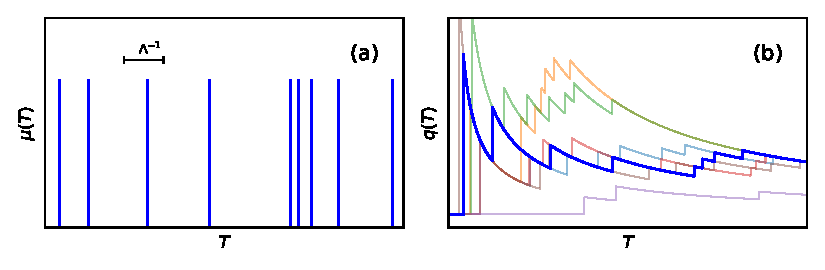
\includegraphics[width=\linewidth,keepaspectratio]{./figures/ch1/anceyRenewal.pdf}
	\caption{The scale-dependent sediment flux is described as a renewal process. Panel (a) indicates the arrivals of particles at rate $\Lambda$, while panel (b) shows an ensemble of realizations of the sediment flux versus the observation time $T$. Note that different realizations of the flux converge toward the same value at large observation times, whereas at small observation times, uncertainty in the flux is large. This is observation-scale dependence. The nature of this convergence depends on the particle dynamics in an as yet unspecified way. }
	\label{fig:ancey}
\end{figure}
Earlier studies have considered different arrival time distributions to calculate the probability distribution of the time-averaged sediment flux, but only the simplest exponential case is reviewed here. The exponential inter-arrival time distribution is $P(t) = \Lambda \exp(-\Lambda t),$ so the rate of particle arrivals is $\Lambda$.
In this case, the flux averaged over a period $T$ can be represented with a Poisson pulse noise, similar to the particle position in the Einstein model of section \ref{sec:einwalk}:
\be q(T) = \frac{1}{T}\int_0^T dt' \mu(t'). \label{eq:flucflux}\ee
Here, the noise is 
\be \mu(t) = \sum_{i=1}^{N(t)}\delta(t-t_i), \label{eq:poissfluxnoise}\ee
as indicated in figure \ref{fig:ancey} panel (a). In this equation, $N(t)$ is Poisson distributed with rate $\Lambda$. 
The flux in eq. \ref{eq:flucflux} is a random variable as indicated in figure \ref{fig:ancey} panel (b). Its probability distribution $P(q|T)$, which is contingent on the observation time $T$, can be derived by evaluating $P(q|T) = \bra \delta(q-\int_0^T \mu(t') dt'/T) \ket$.
This equation entails an average over all possible realizations of the noise in eq. \ref{eq:poissfluxnoise}, producing \citep{VanKampen2007}
\be P(q|T) = \sum_{l=0}^\infty \frac{\big(\Lambda T\big)^l}{l!}e^{-\Lambda T}\delta(q-\frac{l}{T}),\ee
which is a scale-dependent Poisson distribution for the sediment flux across the control surface.

The mean flux derived from this renewal scheme -- $\langle q (T)\rangle = \int_0^\infty dq P(q|T)$ -- is
\be \langle q (T) \rangle = \Lambda, \ee
which is independent of the observation scale, while the magnitude of bedload transport fluctuations scales with $1/T$: 
\be \sigma_q(T)^2 = \frac{\Lambda^2}{T}.\ee
Even this simple model gives a non-trivial conclusion that the relative uncertainty in a measurement of bedload transport depends on the observation time: $\sigma_q(T)/\langle q(T) \rangle \propto T^{-1/2}.$ Our uncertainty in a sediment transport measurement diverges as the observation time becomes short.

A limitation of renewal approaches to calculate the flux is that they do not obviously relate to the dynamics of individual particles. In renewal models as they are phrased now, the inter-arrival time distribution is not based on the underlying mechanics of particle transport.

\section{Summary}

This literature review has indicated that successful bedload transport descriptions have been developed to describe individual particles and bedload fluxes, although many limitations are left in need of further research attention.

All of the works reviewed so far are either mean field models that do not include fluctuations, or stochastic models that calculate probability distributions for the quantities of interest.
The common thread of all of these models is that they take advantage of various devices to side-step the complex interplay of turbulence and granular physics which ultimately control bedload transport.

In the case of mean field models, the devices are heuristic scaling arguments and semi-empirical formulas, while in the case of stochastic models, they are simplified dynamical equations driven by idealized noises, like sequences of pulses, alternating switches, and erratic fluctuations.
This thesis applies the latter methodology to many of the limitations highlighted in the review. An outline of the problems to be addressed follows below.

\section{Outline of the thesis}
\subsection{Problem 1: The scale-dependent flux from individual particle dynamics}

The original model by \citet{Einstein1937} described particle trajectories as a sequence of instantaneous steps. This model was subsequently improved include a finite duration of motion at constant velocity \citep{Lisle1998,Lajeunesse2017}.

In reality, particle velocities fluctuate during movements due to turbulence and particle-bed collisions, so there is a need to go one step further and account also for velocity fluctuations of moving particles in Einstein-type models.

In addition, although the scale-dependent sediment flux has been calculated from renewal models \citep{Turowski2010,Ancey2020}, these approaches are not based on the dynamics of individual particles in transport, so it remains unclear how the sediment flux distribution and its scale dependence originate from the transport characteristics of individual grains.

Chapter \ref{ch:flux} introduces a new model of individual bedload trajectories that includes velocity fluctuations in the motion state. The chapter also demonstrates how these trajectories can be used to calculate the scale-dependent probability distribution of the bedload flux.
This joins together and extends studies from \citet{Einstein1937} to \citet{Ancey2020b} to develop new understanding of individual particle motions and the scale-dependent sediment flux.

\subsection{Problem 2: Feedbacks between sediment transport fluctuations and bed elevation change}

Birth-death models calculate the flux probability distribution assuming that entrainment and deposition do not change the local bed elevation \citep{Heyman2013,Ancey2014}, but this assumption violates conservation of mass.

Bed elevation changes produce sediment burial, and although sediment burial is known to affect tracer particle motions at geomorphic timescales \citep{Ferguson2002,Hassan2017}, our understanding of how long sediment can remain buried is limited.

Chapter \ref{ch:ch3} generalizes the model of \citet{Ancey2008} to include bed elevation changes in order to evaluate the effect of bed elevation change on bedload transport fluctuations and to study how the timescales of sediment burial relate to the movement characteristics of individual grains.

\subsection{Problem 3: The effect of sediment burial on downstream transport of sediment tracers}

Modelling sediment transport as an alterating sequence of motion and rest intervals implicitly assumes that particles are either moving or resting on the bed surface. Although this provides a useful description of bedload transport across local and intermediate timescales, it requires modification to describe for global and geomorphic timescales. 
At longer timescales, particle burial moderates the downstream movements of grains \citep{Hassan2017}, but burial has not yet been incorporated into Einstein-type models of particle trajectories. 

Chapter \ref{ch:downDiff} generalizes the model of \citet{Lisle1998} and \citet{Lajeunesse2017} to include sediment motion, rest, and burial.
This provides the first description of sediment trajectories over local, intermediate, global, and geomorphic timescales.

\subsection{Problem 4: The control of particle-bed collisions over bedload particle velocity distributions}

Finally, the Langevin models of \citet{Fan2014} and \citet{Ancey2014} describe the velocity distributions of sediment moving downstream in the local and intermediate ranges between entrainment and deposition.
These models produce two different end-member sediment velocity distributions, and no mathematical models have been developed that describe the full range of distributions observed in experiments.

Chapter \ref{ch:langevin} presents a stochastic Langevin model including episodic particle-bed collisions formulated by analogy with the theory of granular gases \citep{Brilliantov2004}.
The episodic representation improves on the static Coulomb-like friction representing collisions in earlier models.
The improved model is demonstrated to describe all of the different bedload velocity distributions which have been reported in experiments.


\endinput


An alternative statistical formulation of the sediment flux provides an approximate correspondence between these two definitions \citep{Ancey2006,Furbish2012}.
This hinges on the probability $P[\textbf{u}_p | \textbf{x},t]$ that a particle contacts a control surface $S$ at position $\textbf{x}$ and time $t$ with velocity $\textbf{u}_p$. 
This conditional probability is considered to result from a very large collection of identical systems selected at random moments in their evolution: that is, the conditional probability is an ensemble quantity \citep{Kittel1958}.  

In terms of this ensemble probability, the flux is \citep{Ancey2006}: 
\be q_s = \int_{\text{all } \textbf{u}_p} \int_S P[\textbf{u}_p | \textbf{x},t] \textbf{u}_p \cdot d \textbf{S} d \textbf{u}_p . \label{eq:anceyflux} \ee
In steady conditions, when the probability is independent of time -- $\partial P / \partial t = 0$.

An approximate connection to a control volume flux can be derived by swapping the ensemble average for a spatial average by integrating along a control volume.  
If the control volume is sufficiently long, $L \rightarrow \infty$, it can be seen as a stack of very many independent cross sectional surfaces. 
These comprise a stack of replicas of $\mathcal{S}$, and at an instant, if spatial correlations in bedload transport are weak, each surface constitutes one configuration of particles intersecting $S$ with some set of positions and velocities contributing to $P$. 
One can then define $P$ by counting occurrences along this stack of replica surfaces with an integral across the control volume.

With this concept of replica surfaces in mind, we can formalize the link with symbols. 
Consider $n$ particles distributed throughout a volume at some set of positions $\textbf{x}_i$ with some set of velocities $\textbf{u}_i$, where $i=0,1,\dots, n$,
The cloud of particles can be represented by its (discrete) density in a position-velocity phase space: 
\be \rho(\textbf{x},\textbf{u}_p) = \sum_{i=1}^n M(\textbf{x}-\textbf{x}_i)\delta^3(\textbf{u}_p - \textbf{u}_i). \ee  
Here $M(\textbf{z})$ is a marker function, which is $1$ if $\textbf{z}$ is inside the particle, and $0$ otherwise.
The marker's volume integral is $\int M(\textbf{x}) dV = \nu_p$, the particle volume. 

Using this density at sufficiently large $L$, the conditional probability $P[\textbf{u}_p | \textbf{x}]$ can be written approximately as an integral over the stack of replica surfaces:
\be P[\textbf{u}_p|\textbf{x}] \approx \frac{1}{L} \int_0^L dx \rho(\textbf{x},\textbf{u}_p). \ee
The integral runs along the downstream coordinate, and the equality becomes exact as $L \rightarrow \infty$.
With this swap of ensemble averaging for spatial averaging, the bedload flux becomes 
\be q_s \approx \int_{\text{all} \textbf{u}_p} \int_S \frac{1}{L} \int_0^L dx \sum_{i=1}^n M_a(\textbf{x}-\textbf{x}_i)\delta^3(\textbf{u}_p - \textbf{u}_i) \textbf{u}_p \cdot \textbf{k} dS d \textbf{u}_p = \frac{\nu_p}{L}\sum_{i=1}^n u_i , \ee
so there is some correspondence between the surface and volume definitions of the flux. Yet this is never exact, except in the unphysical case of sediment transport with no spatial correlations (vanishing particle size, discontinuous trajectories). Apparently, the control volume and control surface formulations of the sediment flux are not equivalent, so we see in the literature two parallel streams of research.

\subsection{First extensions of the Einstein model}

Einstein's model provides a physically-based model for individual particle trajectories which includes the essential processes at play over global timescales when particles alternate between movement and rest. Despite its success, it oversimplifies particle transport, and a number of extensions and improvements have been made in the 85 years since its development.

Einstein's model of particle movement seems to have been overlooked for the first several decades after its development, or possibly overshadowed by Einstein's later work, which uses its essential ideas for more obviously practical purposes.
Eventually, curiosity into individual particle motions was re-sparked by cold war studies into the fate of radioactive contaminants in river channels \citep{Crickmore1962, Hubbell1964, Sayre1965,Yang1971}, and later by the need to estimate sediment transport rates from tracer measurements \citep{Yano1969, Todorovic1975, Nakagawa1976, Nakagawa1980, Hassan1991}. In relation to these issues, Einstein's model received a great deal of new attention which generated some generalizations of the model.

The first set of modifications to Einstein's approach in this period concerned the form of the distributions used for step lengths and resting times. Einsteins flume experiments demonstrated that particle step lengths followed exponential distributions \citep{1937}, and this was confirmed by subsequent studies \citep{Yano1969, Nakagawa1976}. Yet these studies were all conducted in steady flows in artificial flumes, not real streams, where sediment transport conditions can be different. When sediment transport is observed before and after a flood, rather than during steady flow, the step lengths are better described by a Gamma distribution, this being the sum across the numerous individual steps that occurred during the flood \citep{Hassan1991}. When sediment transport occurs in the presence of dunes or other bedforms, similar modifications have been made to account for spatial differences in transport characteristics \citep{Crickmore1962, Hubbell1964, Sayre1965} and the embedding of particles within bedforms (which increases the periods of rest) \citep{Yang1971,Nakagawa1980}.

A full statistical characterization of sediment transport is desirable because transport fluctuations are responsible for the initiation of bedforms \citep{Jerolmack2005,Bohorquez2016} and are beginning to show links to basic geomorphology considerations like the maintenance of stable channel widths \citep{Abramian2019,Abramian2020}.
This is not to mention that because sediment transport fluctuations are ubiquitous, models which describe only mean bedload fluxes signals are conceptually incomplete.

An additional reason to characterize fluctuations in bed load fluxes is because in reality, sediment flux measurements always involve a sampling interval.
This introduces questions of the convergence of transport rate measurements \citep{Dhont2018,Ancey2020}.
Fluctuations originate from processes which span a vast range of characteristic timescales.
These can occur over a matter of seconds, such as differences in the velocities of grains due to a series of collisions \citep{Benavides2021}, to many hundreds of hours, such as the migrations of dunes and bedload sheets \citep{Hammamori1962,Hoey1992,Guala2014} or the cycling between aggradation and degradation in pools \citep{Dhont2018}.
Such processes introduce temporal correlations into sediment transport signals which control the sampling interval over which measurements of the mean sediment flux converge \citep{Saletti2015,Singh2009,Singh2012}.
To date, very few modelling works have addressed the observation scale depedence of the bedload flux, whereby measurements of mean fluxes, or statistical moments, shift with observation time \citep{Ancey2020}.


These models produce successful descriptions of disparate experimental results, although their components are not clearly interpretable in terms of physical expecatations. For example, granular interactions were included in the Fan et al model as a Coulomb friction term. While such approximations are common within Earth science models \citep{Kirkby1971}, they are not entirely satisfying given that bedload particles undergo intermittent collisions with the granular bed. Although these motions are sometimes described as ``sliding", bedload particles do not slide in the same sense as a block on a plane, as the granular term in the Fan et al Langevin model indicates.
In a similar way, the Ancey model does not have a particle-particle interaction term, and it includes what is apparently a Stokes drag term (linear in $u-U$), which is not applicable to bedload transport in water, since bedload particles are typically large compared to the viscous length scale \citep{Clift1978}.
We have to wonder if a more detailed treatment of particle-bed interactions might produce a more general model of bedload particle velocities for application at the local and intermediate scales.


One overarching methodology is the use of idealized noises in combination, where each represents a separate mechanical process affecting the movements of particles. This takes on more mathematical complexity than earlier studies, but it also introduces more realism.

Regarding the movements of individual particles, the division into local, intermediate, global, and geomorphic ranges by \citet{Nikora2001,Nikora2002} and \citet{Hassan2017} provides a conceptual scheme by which to organize the current state of research.
Einstein's original description \citep{Einstein1937} and those of his early followers \citep{} described only the global range associated with timescales over which particles cycle through motion and rest.
This limitation was overcome in later works which included a finite duration of sediment motion in order to describe both intermediate and global scales, and Newtonian models have also attained descriptions of additional scales, such as local and intermediate \citep{}.
Meanwhile, Langevin models have derived the velocity characteristics of particles within the local range \citep{}, although they do not manage to account for the full range of experimentally-observed distributions.
The major shortcoming exposed by this framing in terms of the timescales of particle motion is that no models have yet resolved particles across the full set of timescales, so all of these descriptions are essentially incomplete.

Models of the sediment flux face a similar set of shortcomings.
Einstein and Bagnold founded complementary perspectives of the sediment flux. Both were mean field theories, but one counted particles crossing a surface using probabilistic arguments, while the other considered an average energy balance in a control volume.
Research has come a long way since these studies, but the essential divide between surface and volume-based flux calculations still exists. These definitions are not equivalent.
The erosion-deposition model takes steps toward joining these two mean-field theories into a common framework, though it involves many parameters which must be experimentally calibrated.
A paradigm shift in this research stream came from the recognitition that the sediment flux is a fluctuating quantity best characterized by a probability distribution, and from the acknowledgement that measured values of the sediment flux depend on observation scale, meaning it is a scale-dependent quantity.
Although simple models of the sediment flux probability distribution have been developed, they stand somewhat apart from the detailed dynamics of individual particles. Rather than describing particles moving downstream through cycles of entrainment and deposition as in \citet{Einstein1937}, these methods characterize particle motions by herustic entrainment and deposition rates, or interarrival time distributions, which are somewhat abstract objects, not concretely related.
Despite the considerable progress these approaches have brought, the lack of connection to the underlying particle mechanics requires attention.





Alongside this central result $q=E\ell$ for the mean flux, Einstein formulated the entrainment rate $k_E$ of the individual particle in terms of the force balance on the stationary particle, building insight into the grain-scale mechanics of entrainment.
His original approach considers that entrainment is driven by the fluctuating lift force imparted by the turbulent flow, and it is resisted by the submerged weight the grain.
The entrainment rate is calculated from the exceedance probability of the turbulent lift over the weight, providing an alternative to the critical shear stress concept which explicitly incorporates turbulent fluctuations in the fluid flow.
This formulation of entrainment probability in terms of the exceedance of random driving quantities over (possibly
random) resisting quantities \citep{Grass1970} another of Einstein's key contributions.
\citet{Paintal1971} made a significant extension
by including the random supporting geometry of bed particles into the force balance.
More recently, \citet{Tregnaghi2012}
amended the theory to include both force magnitude and duration, incorporating the recognition that both are relevant for particle entrainment \citep{Diplas2008, Valyrakis2013, Celik2014}.
Refined theories of the single-particle entrainment rate, all fundamentally similar to the original ideas of \citet{Einstein1950}, have been carefully reviewed by \citet{Dey2018} and are a topic under active development.

